\icode[magenta]{E-ME-MU-L4-261019-002}
如图所示，一顶角为直角的“\tikz\draw (0,0)--++(45:.4)--++(-45:.4);”形光滑细杆竖直放置，质量均为 \(m\) 的两金属环套在细杆上，高度相同，用一劲度系数为 \(k\) 的轻质弹簧相连，此时弹簧为原长 \(l_0\)。两金属环同时由静止释放，运动过程中弹簧的伸长在弹性限度内，且弹簧始终保持水平，已知弹簧的长度为 \(l\) 时，弹性势能为 \(\frac{1}{2}k(l-l_0)^2\)，重力加速度为 \(g\)，下列说法正确的是\paren[]
	
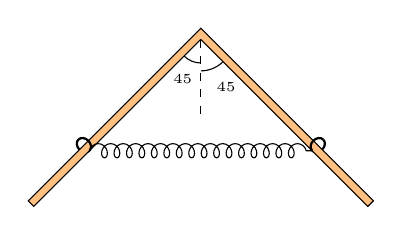
\begin{tikzpicture}
	\draw[rotate=-45,thick] (2,0) arc(-90:90:.08 and .1);
	\draw[rotate=45,thick] (-2,0) arc(-90:-270:.08 and .1);
	\draw[fill=orange!50] (0,0)--++(-135:3)--++(135:.1)--++(45:3.1)--++(-45:3.1)--++(-135:.1)--++(135:3);
	\draw[decoration={aspect=.8,segment length=4.5,amplitude=.9mm,coil},decorate] (-135:2)--(-45:2);
	\draw[rotate=-45,thick] (2,0) arc(270:90:.08 and .1);
	\draw[rotate=45,thick] (-2,0) arc(-90:90:.08 and .1);
	\draw[dashed] (0,0)--(0,-1);
	\draw (0,-.3) arc(-90:-135:.3) (0,-.4) arc(-90:-45:.4);
	\node at (.3,-.6){\tiny \,\qty{45}{\degree}};
	\node at(-.25,-.5){\tiny \,\qty{45}{\degree}};
\end{tikzpicture}
\begin{choices}
	\item 金属环在最高点与最低点加速度大小相等
	\item 左边金属环下滑过程机械能守恒
	\item 弹簧的最大拉力为 \(2mg\)
	\item 金属环的最大速度为 \(g\sqrt{\frac{m}{2k}}\)
\end{choices}
\begin{answer}
    
\end{answer}